\chapter{Entwicklung des Stellwerks}\label{text:Entwicklung-des-Stellwerks}

In den vorangegangen Kapiteln wurde beschrieben, wie die Stellwerkstechnik bei realen Eisenbahnen funktioniert. Das Wissen über Gleisfreimeldeanlagen wurde auf den Kontext einer Klemmbausteineisenbahn übertragen und eine für diesen Zweck geeignete Gleisfreimeldeanlage entwickelt. In diesem Kapitel soll die Entwicklung des Stellwerks beschrieben werden.

Hierfür wird in \autoref{text:Entwicklung-des-Stellwerks:Fahrstrassenlogik} \nameref{text:Entwicklung-des-Stellwerks:Fahrstrassenlogik} auf den Kern des Stellwerks eingegangen, die Bildung und Auflösung von Fahrstraßen. Anschließend wird in \autoref{text:Entwicklung-des-Stellwerks:Signaldecoder} \nameref{text:Entwicklung-des-Stellwerks:Signaldecoder} und \autoref{text:Entwicklung-des-Stellwerks:Weichendecoder} \nameref{text:Entwicklung-des-Stellwerks:Weichendecoder} auf die Ansteuerung der Signale und die Ansteuerung der Weichen eingegangen. Abschließend zeigt \autoref{text:Entwicklung-des-Stellwerks:Bedienung} \nameref{text:Entwicklung-des-Stellwerks:Bedienung} wie das Stellwerk zu bedienen ist.

Das gesamte Kapitel bezieht sich im speziellen auf den in \autoref{abb:Entwicklung-des-Stellwerks:Bahnhof-Gleisplan} dargestellten Gleisplan. Eine umfangreichere Gleisanlage wäre wünschenswert gewesen, war aber aufgrund mangelnden Materials nicht möglich.

\begin{figure}[H]
    \centering
    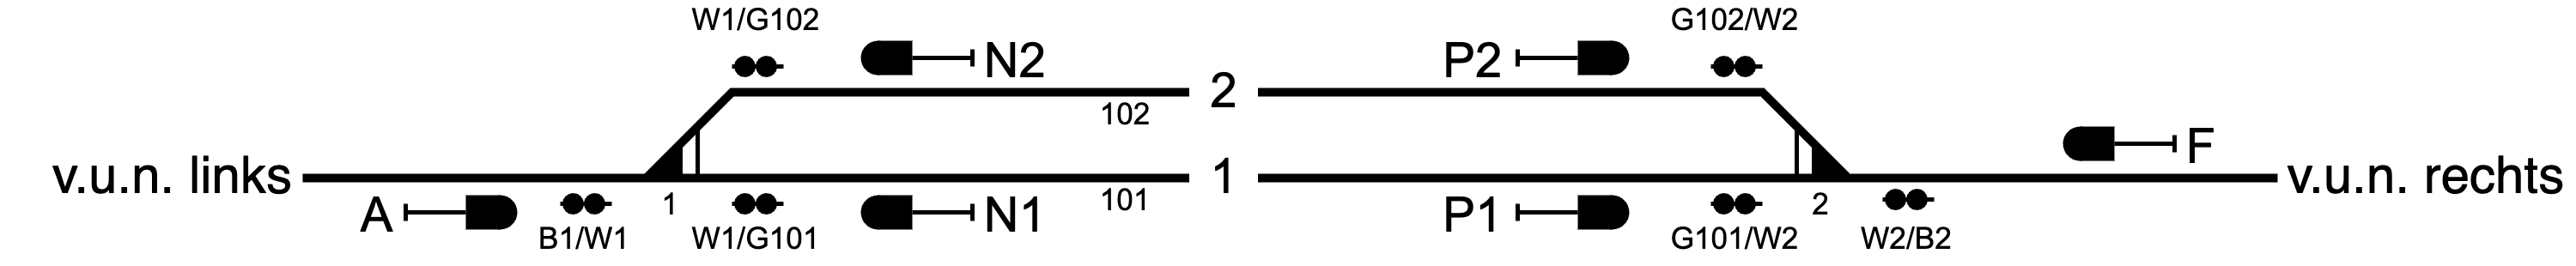
\includegraphics[width=\textwidth]{Assets/Images/5-Entwicklung-des-Stellwerks/Bahnhof-Gleisplan.png}
    \caption{Gleisplan des Bahnhofs}\label{abb:Entwicklung-des-Stellwerks:Bahnhof-Gleisplan}
\end{figure}

Der Bahnhof und alle anderen Elemente wurden mit Steinen des dänischen Klemmbausteinherstellers LEGO\textsuperscript{\tiny{\textregistered}} gebaut.

An dieser Stelle muss erwähnt werden, dass bei der Entwicklung des Stellwerks große Probleme auftraten. Während die Entwicklung der Fahrstraßenlogik und der Gleisfreimeldeanlage weitestgehend reibungslos vonstatten ging, gelang es nicht, die einzelnen Komponenten kommunizieren zu lassen. Daher wurden der Signaldecoder und der Weichendecoder nicht implementiert und können nur konzeptuell behandelt werden. Eine detailliertere Problembeschreibung findet sich in \autoref{text:Entwicklung-des-Stellwerks:Probleme-bei-der-Kommunikation} \nameref{text:Entwicklung-des-Stellwerks:Probleme-bei-der-Kommunikation}.

\newpage
\input{Text/5-Entwicklung-des-Stellwerks/Fahrstraßenlogik.tex}

\newpage
\section{Gleisfreimeldeanlage}\label{text:Entwicklung-des-Stellwerks:Gleisfreimeldeanlage}

In \autoref{text:Methodik:Achszähler} \nameref{text:Methodik:Achszähler} wurden verschiedene technische Umsetzungen von Achszählern für Modelleisenbahnen beschrieben. Für dieses Projekt wurden Reed-Kontakte verwendet, da es sich dabei um die einfachste Umsetzung handelt. Ein Bild eines Testaufbaus ist in \todo{Link} zu sehen.

\todo{Code-Styling}

In \autoref{code:Entwicklung-des-Stellwerks:Gleisfreimeldeanlage:contact-point} ist die zentrale Datenstruktur der Gleisfreimeldeanlage aufgeführt.

\begin{margin}
    \begin{lstlisting}[language=C, label=code:Entwicklung-des-Stellwerks:Gleisfreimeldeanlage:contact-point, caption={Repräsentation eines Kontaktpunktes mit Richtung}]
typedef struct {
    int id;

    rail_contact_point_t *outer; // dieser struct hat nur eine ID
    rail_contact_point_t *inner; // dieser struct hat nur eine ID

    bool is_entering;
    bool is_leaving;
} rail_contact_point_directed_t;
    \end{lstlisting}
\end{margin}

Da für einen Achszähler die Richtung eines Fahrzeugs bestimmt werden soll, enthält der oben aufgeführte gerichtete Achszähler zwei einfache Achszähler, sowie die Information, ob ein Fahrzeug gerade einen Freimeldeabschnitt betritt oder verlässt.

Löst einer der Kontakte aus, wird eine Reihe von unterschiedlichen Konstellationen abgefragt, um herauszufinden, in welche Richtung sich ein Fahrzeug bewegt (also welche Freimeldeabschnitte betroffen sind) und ob diese Bewegung überhaupt möglich ist. Wird eine unlogische Bewegung festgestellt, muss davon ausgegangen werden, dass sich ein Fahrzeug nicht so bewegt wie es soll und unverzüglich ein Fehler an das Stellwerk gesendet werden. Dieses würde dann einen Nothaltauftrag auslösen.


\newpage
\section{Signaldecoder}\label{text:Entwicklung-des-Stellwerks:Signaldecoder}

Der Signaldecoder ist eine Software, die auf einem Raspberry Pi Pico läuft. An ihm sind die LEDs aller Signale direkt angeschlossen. Der Decoder erhält bei der Initialisierung eine Liste all seiner Signale und eine Zuordnung der I/O-Pins zu den LEDs. Anschließend kann er Befehle zum Ansteuern der Signale empfangen.


\newpage
\section{Weichendecoder}\label{text:Entwicklung-des-Stellwerks:Weichendecoder}

Aufgrund der zuvor erwähnten Probleme bei der Kommunikation, wurde auch der Weichendecoder nicht implementiert. Hierfür kann eine mögliche Umsetzung konzeptuell beschrieben werden.

Je nachdem welche Weichen verwendet werden, gibt es verschiedene Möglichkeiten sie zu stellen:

\begin{description}
    \item[Integrierte Steuerung] Im einfachsten Fall wird eine Weiche genutzt, die entweder bereits eine integrierte Steuerung hat, oder aber miteiner solchen nachgerüstet werden kann. Weichen mit integrierter Steuerung gibt es beispielsweise von LEGO\textsuperscript{\tiny{\textregistered}} für das 12V- und 9V-System.
    \item[Elektromagnet] Hat die verwendete Weiche keine integrierte Steuerung und lässt sich auch nicht mit dieser nachrüsten, muss eine eigene Lösung entwickelt werden. Diese Weichen sind für den Handbetrieb konzipiert und haben eine Noppe, auf der ein Stein zum vereinfachten Stellen befestigt werden kann. Eine Möglichkeit ist es, einen Permanentmagneten auf dieser Noppe zu platzieren und in geeignetem Abstand einen Elektromagneten anzubringen. Je nach Polung kann die Weiche gestellt werden.
    \item[LED als Indikator] Die simpelste Lösung ist eine LED, die in der Nähe der Weiche angebracht ist und die gewünschte Stellung anzeigt. Der Anwender muss die Weiche dann manuell in die richtige Stellung bringen und beispielsweise über einen Knopf deren Endlage bestätigen.
\end{description}

Eine mögliche Erweiterung der Weichensteuerung ist die Nutzung von elektrischen Kontakten, die die korrekte Endlage einer Weiche überprüfen. Somit würde die Funktionalität einer realen Weiche recht genau nachgebildet werden.


\newpage
\section{Bedienung}\label{text:Entwicklung-des-Stellwerks:Bedienung}

Der Einfachheit halber wurde auf die Entwicklung einer grafischen Benutzeroberfläche in Anlehnung an ein \ac{ESTW}, verzichtet. Stattdessen wurde eine Kommandozeilenapplikation entwickelt, deren Bedienung an die der ersten \ac{ESTW}s angelehnt ist. \autoref{abb:Entwicklung-des-Stellwerks:Bedienung} zeigt die Oberfläche beispielhaft.

\begin{figure}[H]
    \centering
    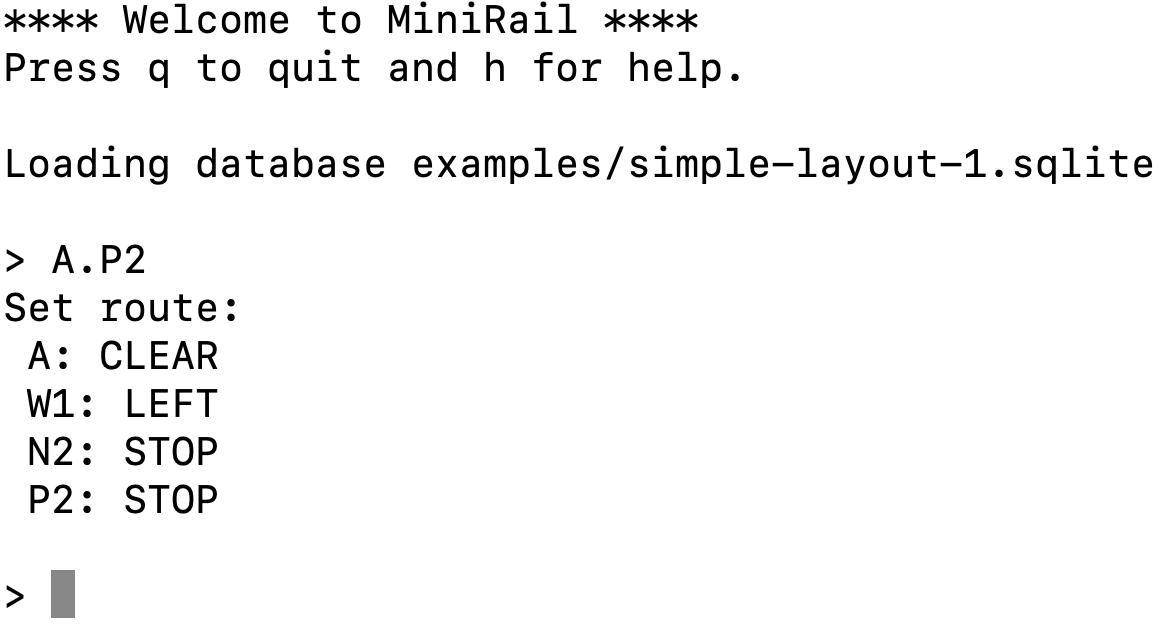
\includegraphics[width=.8\textwidth]{Assets/Images/5-Entwicklung-des-Stellwerks/Bedienung.png}
    \caption{Bedienoberfläche des Stellwerks}\label{abb:Entwicklung-des-Stellwerks:Bedienung}
\end{figure}

Die Topologie der Gleisanlage ist in einer SQLite-Datenbank gespeichert, welche beim Programmstart übergeben wird. Über einen \textit{Bedienstring} wird das Stellwerk gesteuert. Die Syntax ist hier immer \texttt{<start>.<ziel>} und hat das Stellen einer Zugfahrstraße von \texttt{start} nach \texttt{ziel} zur Folge.

Da die einzelnen Komponenten nicht miteinander kommunizieren können, handelt sich die Ausgabe um eine Simulation. Signale und Weichen werden also nicht wirklich gestellt.


\newpage
\section{Probleme bei der Kommunikation}\label{text:Entwicklung-des-Stellwerks:Probleme-bei-der-Kommunikation}

In \autoref{text:Methodik:Kommunikation} \nameref{text:Methodik:Kommunikation} wurde erläutert, wie die einzelnen Komponenten des Stellwerks miteinander kommunizieren können. Zunächst wurde ein CAN-Bus aufgebaut, der über eine USB-Brücke mit dem Computer über eine serielle Schnittstelle verbunden ist. Hierbei wurde beobachtet, der Bus an sich nur selten funktioniert. Das Fehlerbild beschränkt sich auf ein Volllaufen des Puffers beim Sendern einer Nachricht. Es wurde weiter festgestellt, dass der Fehler nicht deterministisch ist, da in manchen Fällen Daten gesendet und empfangen werden können.
Zu Testzwecken wurde der in \autoref{text:Methodik:Kommunikation:CAN-Bus} \nameref{text:Methodik:Kommunikation:CAN-Bus} dargestellte Testaufbau zweier Raspberry Pi Picos (\autoref{abb:Methodik:Kommunikation:CAN-Bus}) an die USB-Brücke angeschlossen. In seltenen Fällen gelang es, die Kommunikation beider Picos auf dem Computer mitzulesen. In der Regel stoppte der Bus, sobald man die Brücke angeschlossen hat.
Erst dann fiel auf, dass selbst jener Testaufbau nur selten funktioniert. Die Theorie, dass die Kontakte der Breadboards nicht sauber geschlossen werden, konnte weder bestätigt, noch widerlegt werden.

Als Notlösung wurde anschließend versucht, mit UART eine Art Bus zu simulieren (siehe \autoref{text:Methodik:Kommunikation:UART} \nameref{text:Methodik:Kommunikation:UART}). Hierbei kam es zu diversen Problemen, unter anderem dem Senden von Phantom-Bytes und der Kodierung empfangener Daten. Daher musste auch dieser Ansatz verworfen werden.

